
\subsection{Persistence optimization}\label{sec:persistence-optimization}


Leftover signal (``persistence") in the first dark image acquired after intense illumination has
been observed Section \ref{sec:initPersistenceChar}.  Persistence has been observed
in an early prototype e2v sensor as early as 2014
\citep{2014SPIE.9154E..18D}. It was confirmed that the amplitude of
the persistence decreased as the parallel swing voltage was decreased.
This is consistent with the persistence being a Residual Surface Image (RSI) effect as described in
\citet{2001sccd.book.....J}, i.e., the excess charges are being trapped
at the surface layer. The level of persistence is about 10--20 ADU,
and the decay time constant is about 30\,s
\citep{dmtn-276}.

During the EO testing in 2021 (Run 13177, for example, Run 5), we also found the persistence made a
streak toward the readout direction from the place where a bright spot illumination occurred 
in a previous image. We call this ``trailing persistence".

As noted in Section \ref{sec:divisadero:init}, depending on operating conditions e2v sensors have another major non-ideality, so-called ``tearing", which is
considered a consequence of the non-uniform distribution of holes. Over the past few years, our
primary focus in the optimization of the operating parameters was mitigation of the tearing, and we successfully eliminated the tearing by changing the
e2v voltages from unipolar (both parallel rails high and low
are positive) to bipolar (the parallel high is positive, and
the low is negative) following \href{https://github.com/lsst-camera-dh/mkconfigs/blob/master/newformula.py}{the Bipolar voltage formula}.
However, the persistence issue
remained unchanged.

For the persistence issue, if this is a residual surface image, two
approaches could be taken as discussed in \citet{2024SPIE13103E..0WU}:  
either 1) establishing the pinning condition where the holes make a thin
layer at the front surface so that the excess charges recombine with
the holes, or 2) narrowing the parallel swing so that the accumulated
charges in the silicon do not get close to the surface state.

The pinning condition could be established by decreasing the parallel low
voltage to as low as -7.0\,V or lower. The transition voltage needs to be
empirically determined. However, Teledyne e2v advised that the measured
current flow increases as the parallel low voltage is decreased, which
increases the risk of damaging the sensor by inducing a
breakdown\footnote{We note that ITL operates at a parallel low voltage
  of $-$8.0\,V. We have observed the increased current flow. But we have
  software protection so that the current does not increase too much.}.
Also, the excess charges could be recombined by the thin layer of
 holes, which could affect linearity at high flux levels when
charges start to interact with the holes.

The parallel swing determines the full-well. Depending on whether the
accumulated charges spread over the columns or interact with the surface
layer, there are blooming full-well regimes and the surface full-well
regime. A full-well level between these two regimes is considered to be
optimal \citep{2001sccd.book.....J}, with no persistence and dynamic range as great as
possible. Because we observe the persistence effect, we likely operate the sensor in the
surface full-well condition and we need to decrease the parallel swing to
get the blooming full-well or the optimal full-well. The obvious downside is
decreasing the full-well capacity.

The sensor control voltages are defined relative to each other. Changing, e.g., the parallel
swing also requires changes to all other voltages to
operate the sensor properly, e.g., to properly reset the amplifier.
The initial voltages were given in the original Bipolar formula
 but to decrease the parallel swing we had
to switch to the new persistence mitigation formula in order to satisfy the constraints (\href{https://github.com/lsst-camera-dh/e2v_voltages/blob/main/setup_e2v_v4.py}{Persistence mitigation voltage}).

\citet{2024SPIE13103E..21S}, set up a single sensor test-stand at UC
Davis. They attempted multiple different approaches mentioned above and
reported the results in \citet{2025arXiv250205418P}. 
The summary is as follows:

\begin{itemize}
\tightlist
\item
  The new voltages following the persistence mitigation voltage rule produces reasonable bias, dark, flat images visually.
\item
  Narrowing the parallel swing eliminates the persistence.
\item Just decreasing the collecting voltage (PclkH) even without changing swing will decrease persistence as the charge packet is not pulled as close to the surface. 
\item
  Lowering the parallel low voltage did not work
  as we expected; going to a more negative voltage is probably needed.
  \end{itemize}

Note that the e2v sensor in the UCD setup did not exhibit the same magnitude of persistence as the LSST Camera.
This might be due to the characteristics of the sensor, or perhaps
the differences in the electronics (e.g., the long cable between CCD and REB). They need to move the both parallel high and low up to reproduce persistence as the similar as the main Camera.

\subsubsection{Persistence optimization}\label{persistence-optimization-1}
Based on this test result, we decided to test the new voltages with
the narrower parallel swing on the LSST Camera focal plane. Keeping the
parallel low voltage at -6.0\,V in order to operate the sensor safely (very
conservative limit), we changed the parallel swing voltage from 9.3\,V to
8.0\,V as well as all the other voltages using the new formula. We
overexposed the CCDs and took 20 darks afterward. Figure~\ref{fig:peristence-swing} compares the
mean and median of pixel-by-pixel differences between the first and the
last dark exposures, as a function of the parallel swing (We note that this is not the persistence metric defined in Sec.~\ref{sec:initPersistenceChar}, but almost identical).
As the parallel swing is decreased, the residual signal decreases, reaching
roughly 10$\times$ less than the original level at 9.3\,V. Although we sampled
at 8.0 (E1363), 8.4 (E1430), 8.65 (E1411), 8.8 (E1424)and 9.3\,V (E1110), 8.0\,V appears to work the best and could
be lower with the penalty of decreasing the full-well capacity.

\begin{figure}[ht]
\begin{centering}
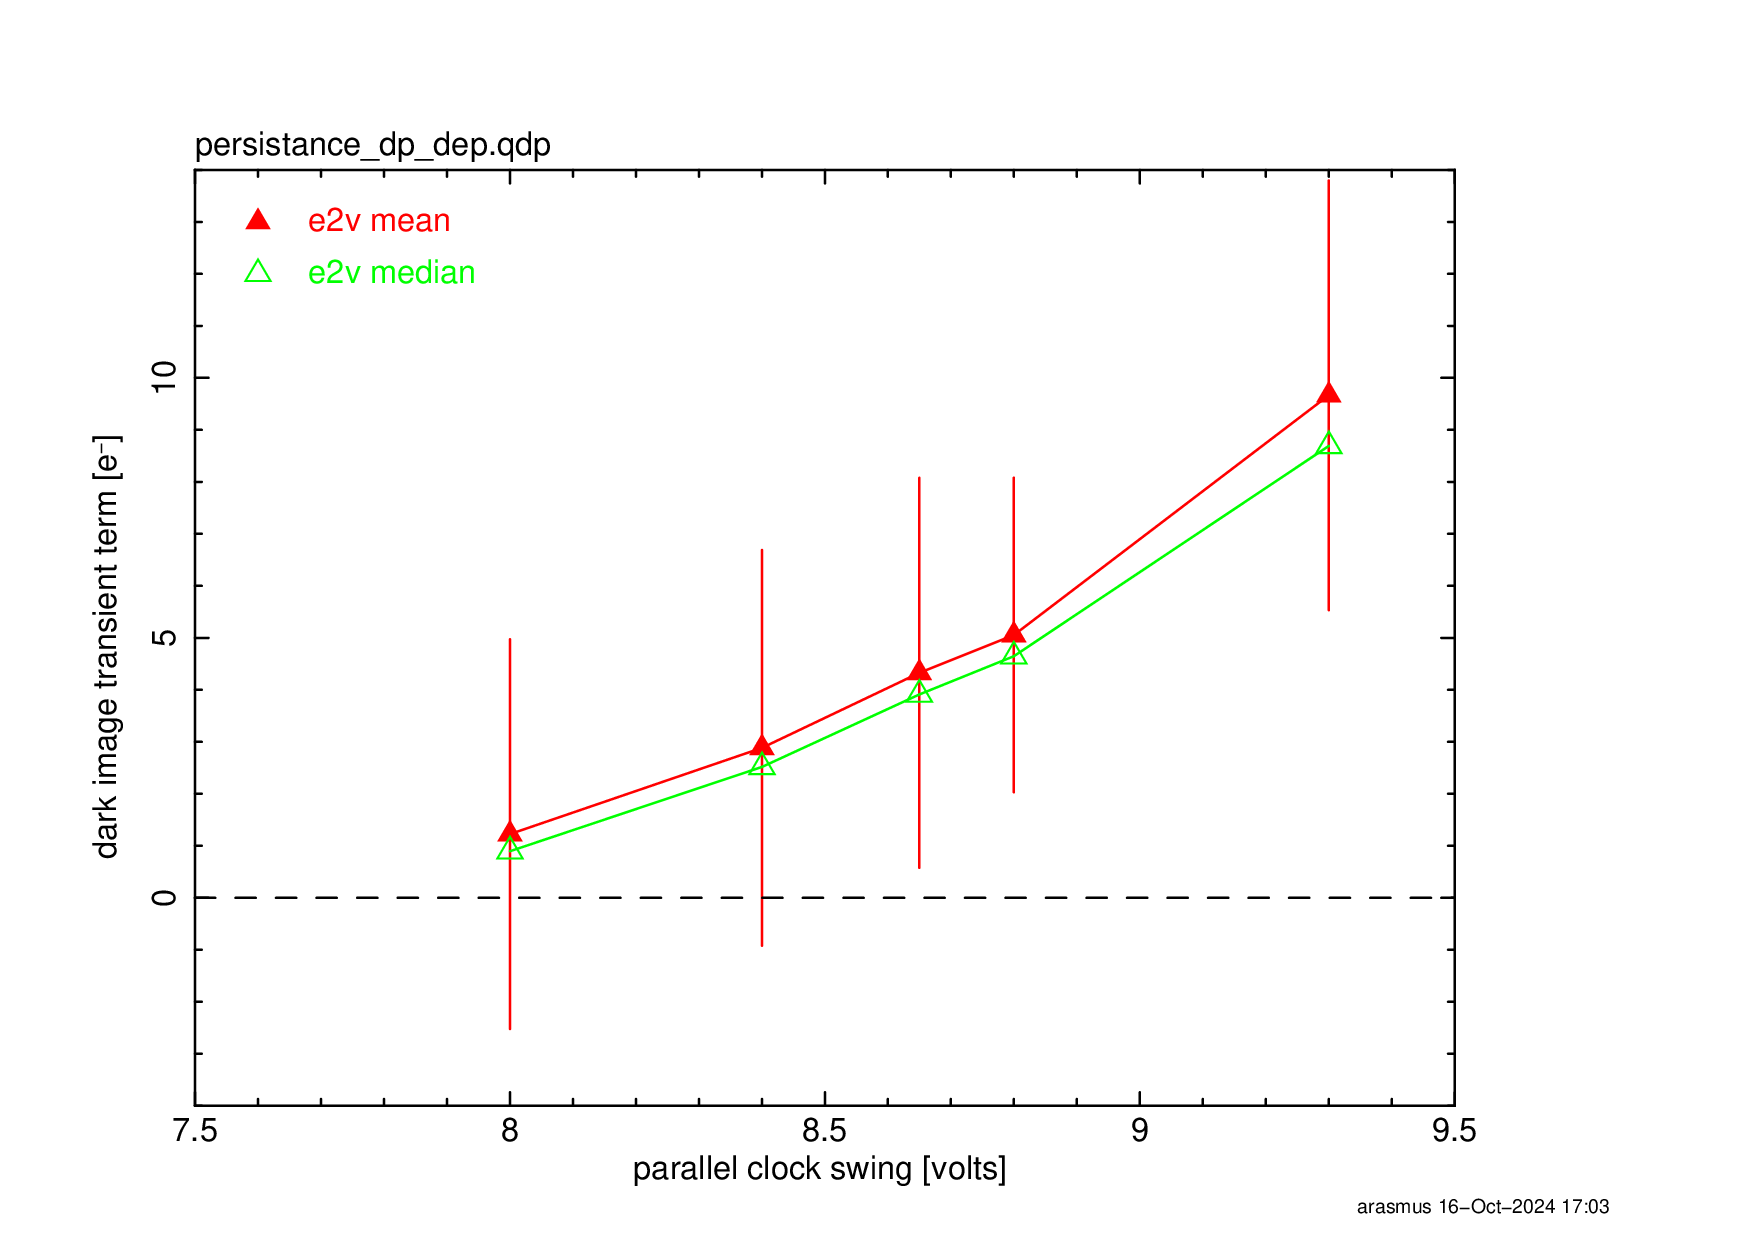
\includegraphics[width=0.9\textwidth]{figures/e2v_transient_dark_vs_dp.png}

\caption{The remaining charges measured in every amplifier but
aggregated by mean and median as a function of the parallel clock swing
are shown.}
\label{fig:peristence-swing}
\end{centering}
\end{figure}

Figure~\ref{fig:persistence-reduction} displays how the persistence is reduced by the
parallel swing decrease. The images were processed with the standard instrumental
signature removal and assembled in the full focal-plane view. The
dark exposure was taken immediately after a 400\,ke-equivalent flat exposure.
The figure shows the distinct pattern of elevated signal associated with
the e2v sensors, which fill the inner part of the focal plane.

The right-hand figure shows the same dark exposure but taken with the narrow
parallel swing voltage of 8.0\,V. The distinct pattern goes away. This
demonstrates the persistence in e2v sensors becomes the (low) level of the 
ITL sensors.


\begin{figure}[ht]
\centering
\begin{minipage}[b]{0.45\textwidth}
\centering
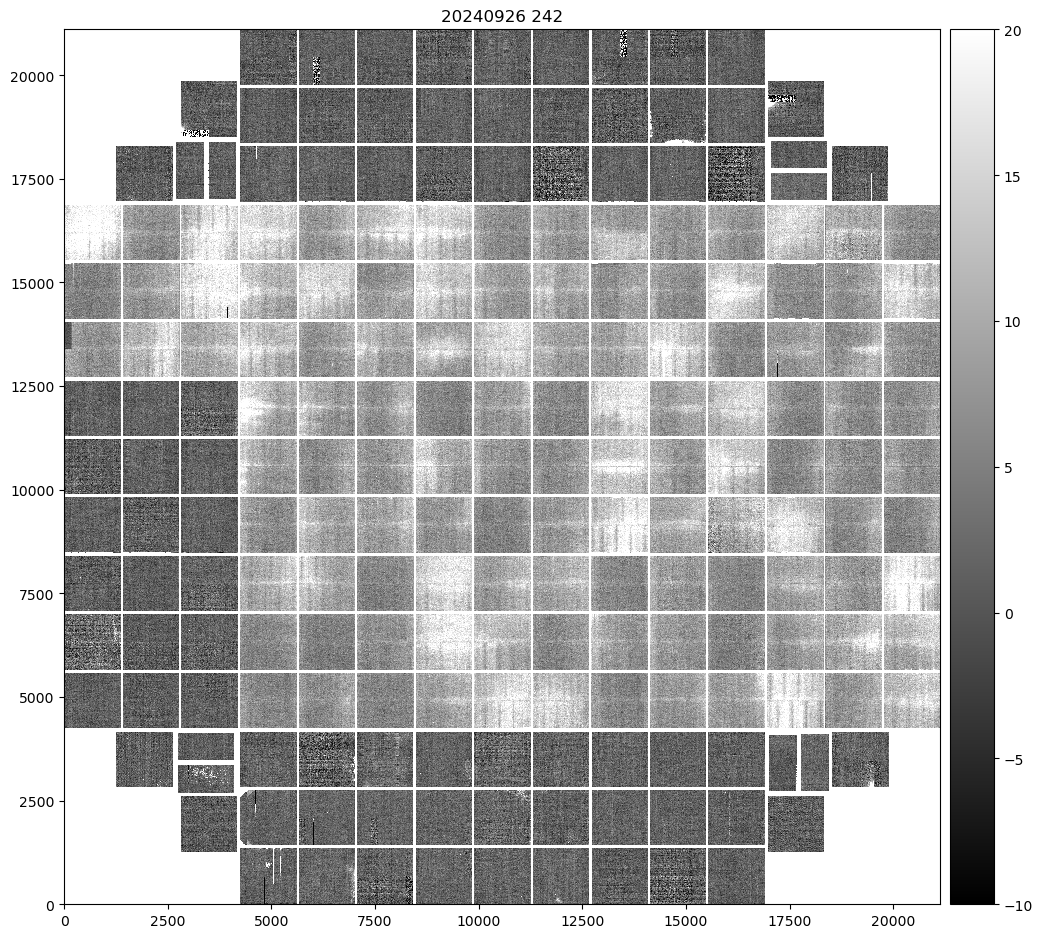
\includegraphics[width=\textwidth]{figures/E1110dp93.png}
\end{minipage}
\hfill
\begin{minipage}[b]{0.45\textwidth}
\centering
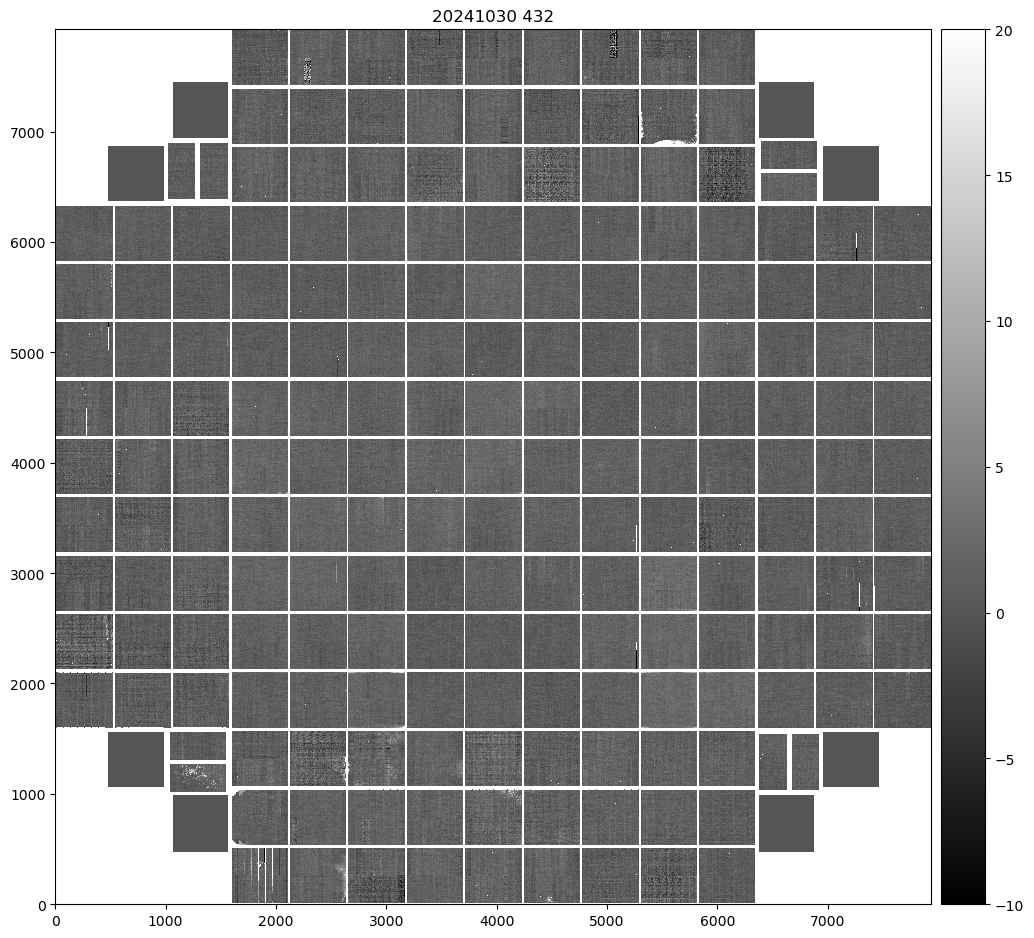
\includegraphics[width=\textwidth]{figures/E1880dp80.png}
\end{minipage}
\caption{Comparison of dark exposures under different parallel swings. (left) The first dark exposure after a 400\,ke$^-$ flat image under the parallel swing of 9.3\,V (Run E1110); (right) The first dark exposure after a 400\,ke$^-$ flat image under the parallel swing of 8.0\,V (Run E1880). The figure shows no distinct patterns from persistence in e2v sensors. Note that the guide sensors were not displayed here because they were being operated in guider mode. Also some of the residuals caused by defects in ITL sensors disappeared here because of the employment of the new sequencer file (v30).}
\label{fig:persistence-reduction}
\end{figure}



\subsubsection{Impact on full-well}\label{impact-on-full-well}

Reduction of the full well is expected from narrowing the parallel swing
voltage. This subsection explores how much reduction in the PTC turnoff
is observed in the dense PTC runs. Two runs were acquired with identical
settings except for the CCD operating voltage (E1113 for 9.3\,V and E1335
for 8.0\,V). As the PTC turnoff is defined in ADU, it needs to be
multiplied by PTC\_GAIN to compare the turnoff values in electrons.
Figure~\ref{fig:ptc-turnoff} compares the PTC turnoffs in electrons and also shows their
fractional difference. The medians of the peaks are 133,065e$^-$, 102,728e$^-$, and the median reduction was 22\%.

\begin{figure}[ht]
\begin{centering}
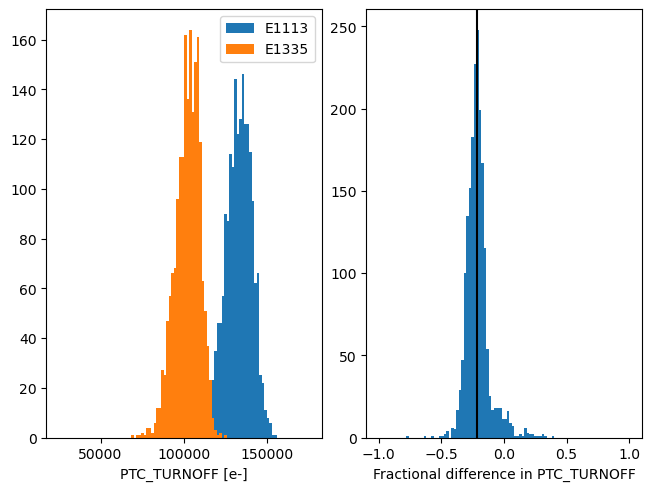
\includegraphics[width=0.9\textwidth]{figures/PtcTurnoffRatio.png}
\end{centering}
\caption{Histograms of the PTC turnoff values scaled to electron units (left) and the ratios of
differences (right) between E1113 (9.3\,V) vs. E1335 (8.0\,V). The reduction of
the median is 23\%.}
\label{fig:ptc-turnoff}
\end{figure}



\subsubsection{Impact on brighter-fatter effect}\label{impact-on-brighter-fatter-effect}

Reducing the parallel swing is expected to enhance the brighter-fatter
effect (BFE), possibly in an anisotropic way. The BFE can be
characterized via the evolution of the variance and covariances of
flat field exposures as a function of flux, i.e., via a PTC analysis. To evaluate the
impact of reducing the parallel voltage swing on e2v sensors, we
acquired two series of flat field exposures with the respective voltage
setups and extracted the ``area" coefficients $a_{ij}$
\citep[Equation (1) in][]{2023A&A...670A.118A}.
The area coefficients describe how much a unit charge stored in
a pixel will alter the area of some other pixel (or itself). We find that
reducing the parallel swing from 9.3\,V to 8.0\,V typically increases the
area coefficients by 10\% (between 5 and 19\% depending on distance indexed by $i,j$),
and the increase is almost isotropic (i.e., very similar along serial and parallel
directions; see Fig.~\ref{fig:area-coeffs}). From these measurements, we anticipate that the increase of
star sizes with flux in LSST data will not become more anisotropic at 8.0\,V than it was at
9.3\,V, and hence this reduction of parallel swing does not 
risk increasing systematic uncertainty of the PSF ellipticity.

\begin{figure}[ht]
\begin{centering}
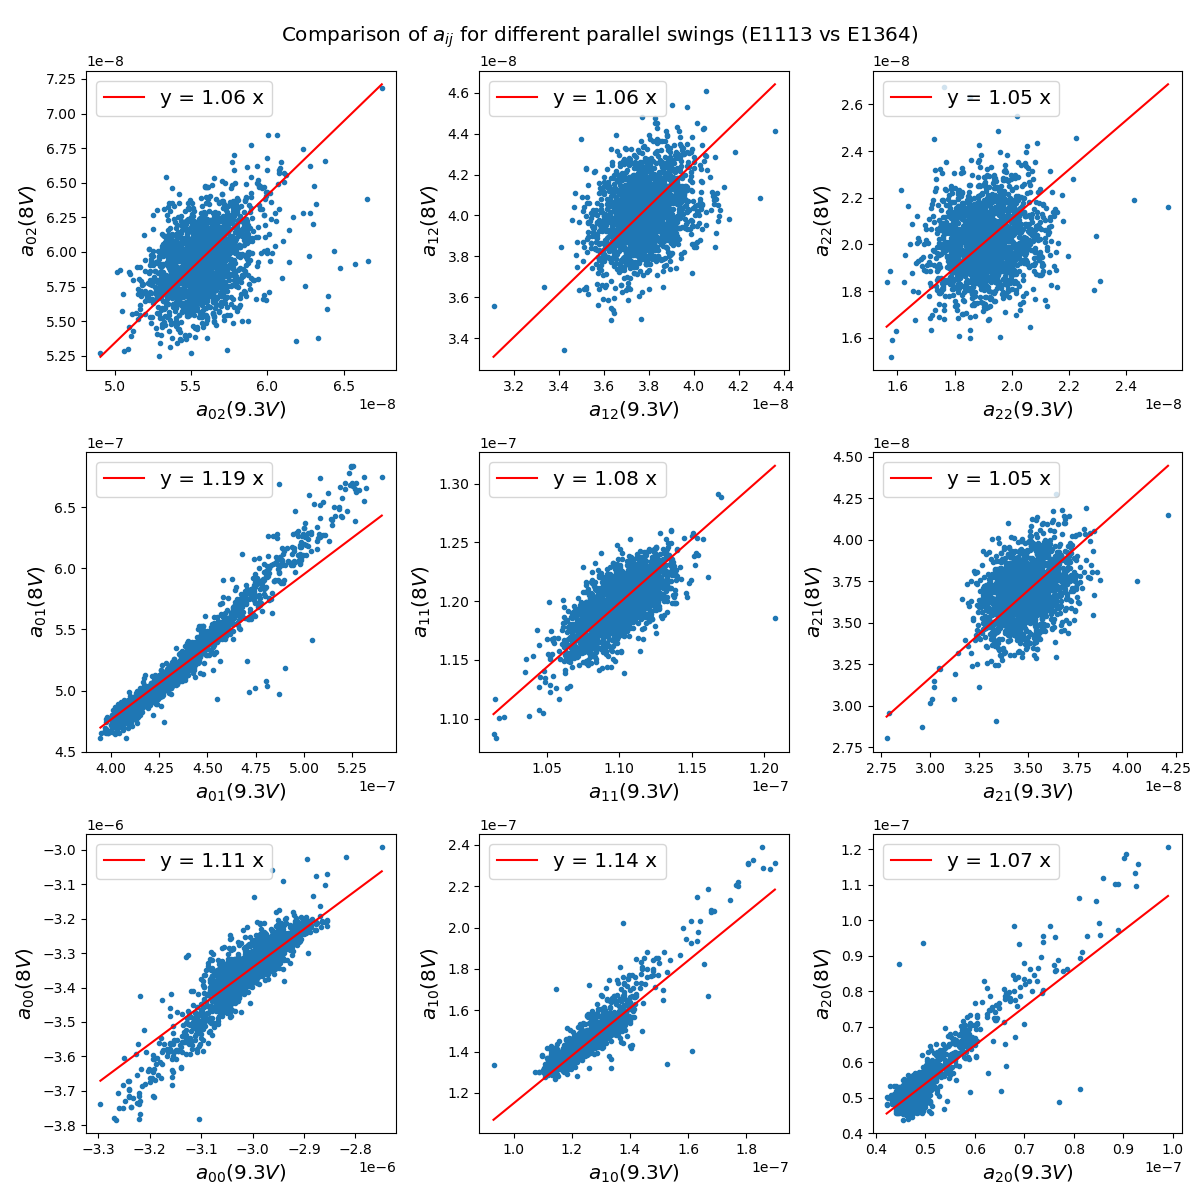
\includegraphics[width=0.8\textwidth]{figures/aScatterPlots8vs9-3.png}
\end{centering}
\caption{Scatter plots of area coefficients $a_{ij}$ (one entry per amplifier)
measured at 8.0\,V and 9.3\,V. The sub-figures correspond to separations in rows ($j$) and columns ($i$)
between the source of the area distortion and its target, with the self
interaction coefficient $a_{00}$ at the bottom left. The first neighbors increase
respectively by 19\% in the parallel direction and by 14\% in the serial
direction. So the BFE is slightly greater at 8.0\,V but not dramatically
more anisotropic: the ratio of parallel to serial nearest-neighbor correlations increases only from 3.43 to 3.54 with the reduction of the parallel swing.}
\label{fig:area-coeffs}
\end{figure}


\subsection{Sequencer optimization}\label{sequencer-optimization}
Several efforts were undertaken to optimize the sequencer configurations during Run 7. The following points summarize the key investigations:

\begin{itemize}
\item {\bf Clear}: Addressing the leftover charges at the image/serial register. The discussion is provided in Section \ref{sec:improved-clear}.
\item {\bf Whether toggling the RG output during the parallel transfer for the e2v sensors is needed}: As such configuration flatten the bias shape for ITL device, the same type of configuration has been tested for e2v sensors during run 7 . Details are provided in Section~\ref{noRGe2v}
\item {\bf Whether running IDLE\_FLUSH is needed}: Whether running IDLE\_FLUSH had an effect on the tearing. Details are presented in Section~\ref{section:disablingIDLEFLUSH}
\item {\bf Phase overlap during parallel transfer for e2v}: e2v sensors feature four parallel phases. To improve the uniformity of the full well across a sensor, overlapping two phases during each time slice of the parallel transfer was introduced.
\begin{itemize}
    \item Sequencer files that are based on the regular v29 but have changes in the parallel transfer by having a half overlap of what it was in the original (\_halfoverlapping.seq), a small amount of overlap compared to what it was in the original (\_overlap113.seq), and overlapping at all (\_nonoverlapping.seq) are created.
    \item Any overlap is known to cause trailing persistence \citep{2025arXiv250205418P}. We conducted several runs using both half-overlapping (E1245) and non-overlapping (E1396) sequencers but we have not studied these because the trailing persistence is no longer a concern after optimizing the operating voltages to avoid charge trapping. 
\end{itemize}


\end{itemize}

\subsubsection{Improved clear}\label{sec:improved-clear}

\paragraph{Overview}\label{overview}

In this section, we describe the work done during Run 7 to improve
the image clear prior to collecting a new exposure.

The problem we wanted to address is the presence of residual charges in
the first rows read for an image taken just after the clear of a saturated
image. These ``hard to clear" charges are associated with highly
saturated flats or columns (or stars as observed in AuxTel or ComCam),
which leave signal in the first row of the subsequent exposure. The effect has a sensor-specific signature:

\begin{itemize}
\item
  For all ITL CCDs (except R01\_S10 for which the effect is much more significant and which will be addressed later in this section): After a very bright exposure that saturates the overscan, the first row of the subsequent image has residual charges which are close to saturation. In most cases a small leftover signal in the second row is also present.
\item
  For e2v CCDs: the first row read after an exposure that follows an exposure with saturated
  overscan, has residual charges which are close to saturation, and a significant signal is present
  in the subsequent 20--50 rows (see left-hand plot in Figure~\ref{fig:clear_e2v}).
  The effect is slightly amplifier dependent.
\end{itemize}

These leftover electrons are not associated with what we usually call residual image or persistence. They are suspected to be associated with pockets, induced by the electric field configuration in the sensor and the field associated with saturated pixels.
Investigation has revealed that only the first exposure taken after an image with saturated overscan is impacted. Our standard clear is not able to flush away those charges, while a standard readout of $\gtrsim$ 2000 rows does remove them.
There is a chance that a change of the electric field (e.g., a change in the clocking scheme defined in sequencer files) can remove the pockets, and free the charges, allowing them to be cleared.

The location of these uncleared electrons in the first row of the
CCDs indicates that the pockets are in the interface between the image area and the serial register. For this reason we investigated
changes in the electric field configuration of the serial register during the
clear, to avoid generating pockets at the image-serial register interface.


To address this clear issue, we focused on updating the serial
register field as the rows are moved into it. The constraint is that
the changes introduced should not significantly increase the clear
execution time. It should be noted that in 2021 we tried a sequencer
called ``Deep Clear" \href{https://github.com/lsst-camera-dh/sequencer-files/blob/master/run5/FP_E2V_2s_ir2_v23_DC.seq}{sequencerV23\_DC} as a first attempt to address the clear issue; it added one full row 
flush on top of the existing one at the end of the clear. This sequencer
did improve the clear, but did  not fully fix the clear issue (see
Table~\ref{tab:clears}).

\clearpage
{\tiny
\begin{longtable}[tbh]{|p{0.2\linewidth}|p{0.12\linewidth}|p{0.2\linewidth}|p{0.2\linewidth}|p{0.2\linewidth}|}
\caption{Clear methods used so far. \label{tab:clears}} \\
\hline
\textbf{Clear Type} & \textbf{Duration (ms)} & \textbf{e2v after Saturated Flat} & \textbf{ITL after Saturated Flat} & \textbf{R01\_S10 ITL ``unique"} \\
\hline
\endfirsthead

%\hline
%\textbf{Clear Type} & \textbf{Clear duration} & \textbf{``E2V" after saturated Flat} & \textbf{``ITL`` after saturated Flat} & \textbf{R01 ITL ``unique"} \\
%\hline
\endhead

\hline
\endfoot

\hline
\endlastfoot

\textbf{Default Clear} 1~clear (seq. V29) & 65.5 & First row saturated signal up to row 50 & 1st row saturated signal up to 2nd row & First 500 rows saturated for 4 amps, 13 amps with signals \\
\textbf{Multi Clear} 3~clears (seq. V29) & 196.5 & No residual electrons & No residual electrons & First 150 rows saturated for 2 amps, 5 amps with signals \\
\textbf{Multi Clear} 5~clears (seq. V29) & 327.4 & No residual electrons & No residual electrons & First 100 rows saturated for 2 amps, 2 amps impacted \\
\textbf{Deep Clear} 1~clear (Seq. V23 DC) & 64.69 & 1st row saturated signal up to row <20 & Tiny signal left in the first row & not measured \\
\textbf{No Pocket (Nop)} 1~clear (seq. V29) & 65.8 & signal up to row 20 & No residual electrons & First 1000 rows saturated for 16 amps, 16 amps with signals \\
\textbf{No Pocket Serial Flush (NopSf)} 1~clear (seq. V29, V30) & 67.0 & No residual electrons & No residual electrons & first 750 rows saturated for 16 amps, 16 amps with signals \\
\end{longtable}
}

\paragraph{New sequencers}\label{new-sequencers}
In Run 7, we considered two new configurations on top of the default clear. The changes are in the ParallelFlush function, which
moves the charges from the image area to the serial register:

\begin{itemize}
\tightlist
\item
  The default clear (V29): In the default clear, all serial clock voltages are
  kept high as the parallel clocks move charges from the image area to the
  serial register (\href{https://github.com/lsst-camera-dh/sequencer-files/blob/master/run7/FP_E2V_2s_l3cp_v29.seq}{sequencerV29}).
  The charges on the serial register are expected to flow to the ground;
  the serial register clocks being held all high, without pixel boundaries, and
  with the Reset Gate of the amplifiers On. At the end of the clear, a full
  flush of the serial register is done.
\item
  The No-pocket Clear (Nop): a clear where the serial register has the
  same configuration (S1 \& S2 high, S3 low) when the parallel clock P1
  moves the charges to the serial register from the image region. We kept all phases up for the rest of the time for a fast clear
  of the charges along the serial register
  (\href{https://github.com/lsst-camera-dh/sequencer-files/blob/master/run7/FP_E2V_2s_l3cp_v29_Nop.seq}{sequencerV29\_Nop}). The idea is
  that the S3 phase is not designed to be high when charges are transferred
  to the serial register, and is probably playing a major role in the creation of pockets.
\item
  The No-Pocket with Serial Flush Clear (NopSf): this sequencer is close
  to the Nop solution, except that during the transfer of one row to
  the serial register, the serial phases are also manipulated to transfer two
  pixels along the serial register. The changes in electric field at the
  image-serial register interface are then even more representative of
  what a standard read produces, and should further prevent the
  creation of pockets.
  (\href{https://github.com/lsst-camera-dh/sequencer-files/blob/master/run7/FP_E2V_2s_l3cp_v29_NopSf.seq}{sequencerV29\_NopSf}).
\end{itemize}


\paragraph{Results for standard e2v and ITL CCDs}\label{results-on-standard-e2v-and-itl-ccd}

\begin{figure}[ht]
\begin{centering}
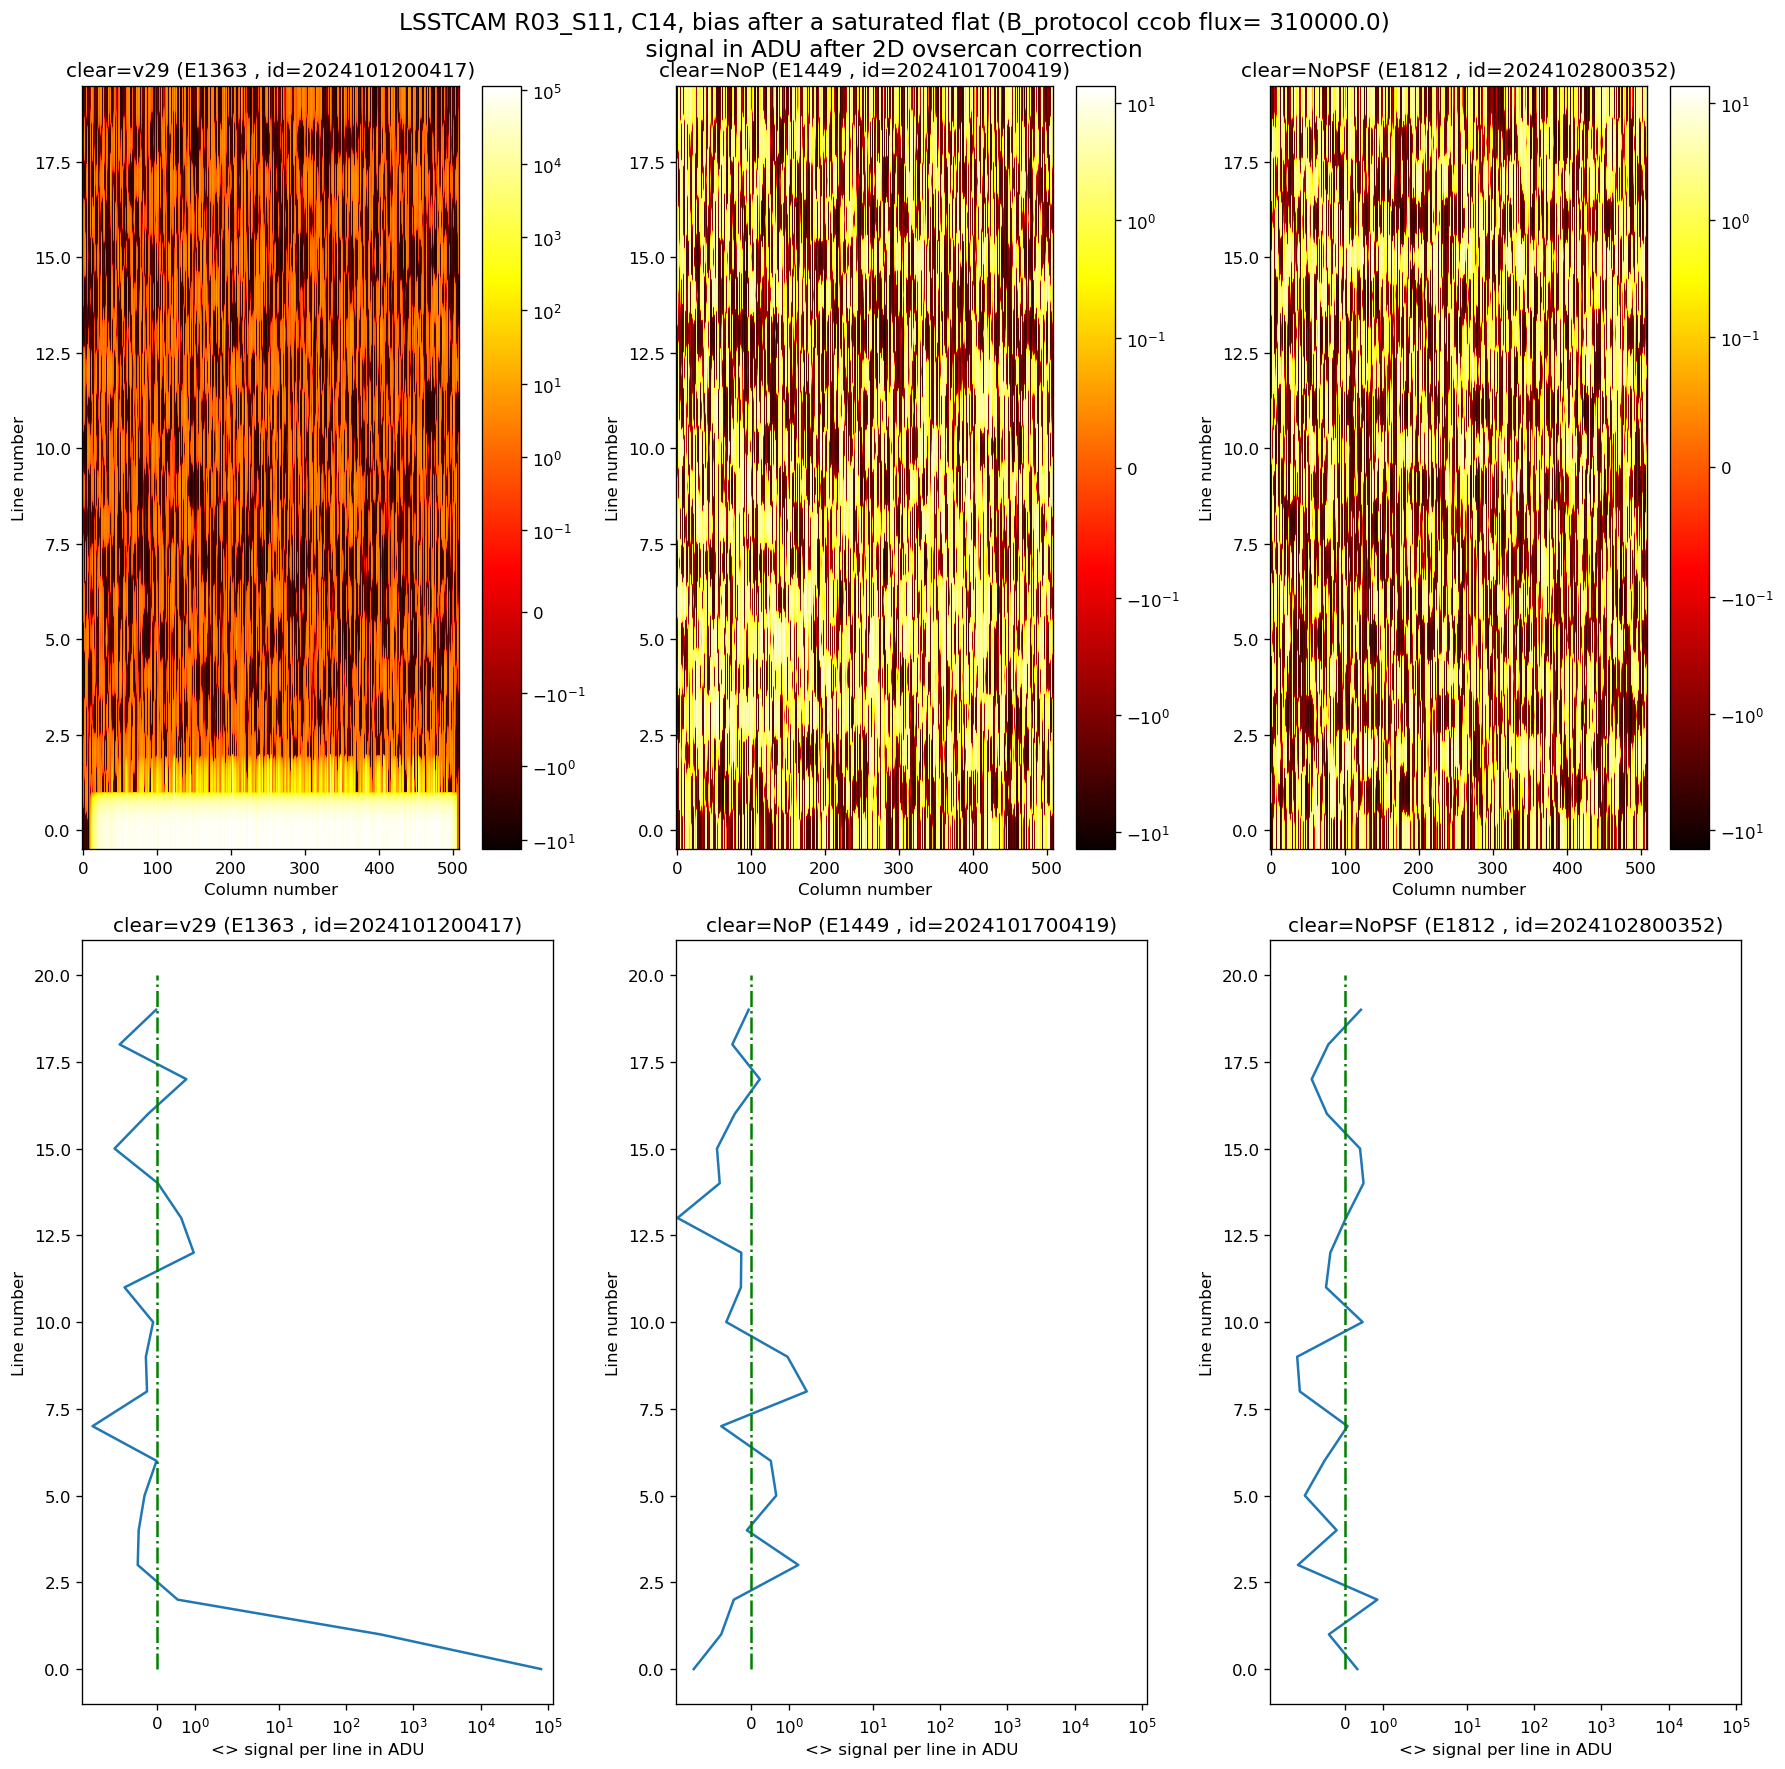
\includegraphics[width=0.9\textwidth]{figures/plots_R03_S11_C14_E1812_bias_2024102800352.png}
\end{centering}
\caption{Same as Figure \ref{fig:clear_e2v} but for an ITL sensor (R03\_S11).}
\label{fig:clear_ITL}
\end{figure}

\begin{figure}[ht]
\begin{centering}
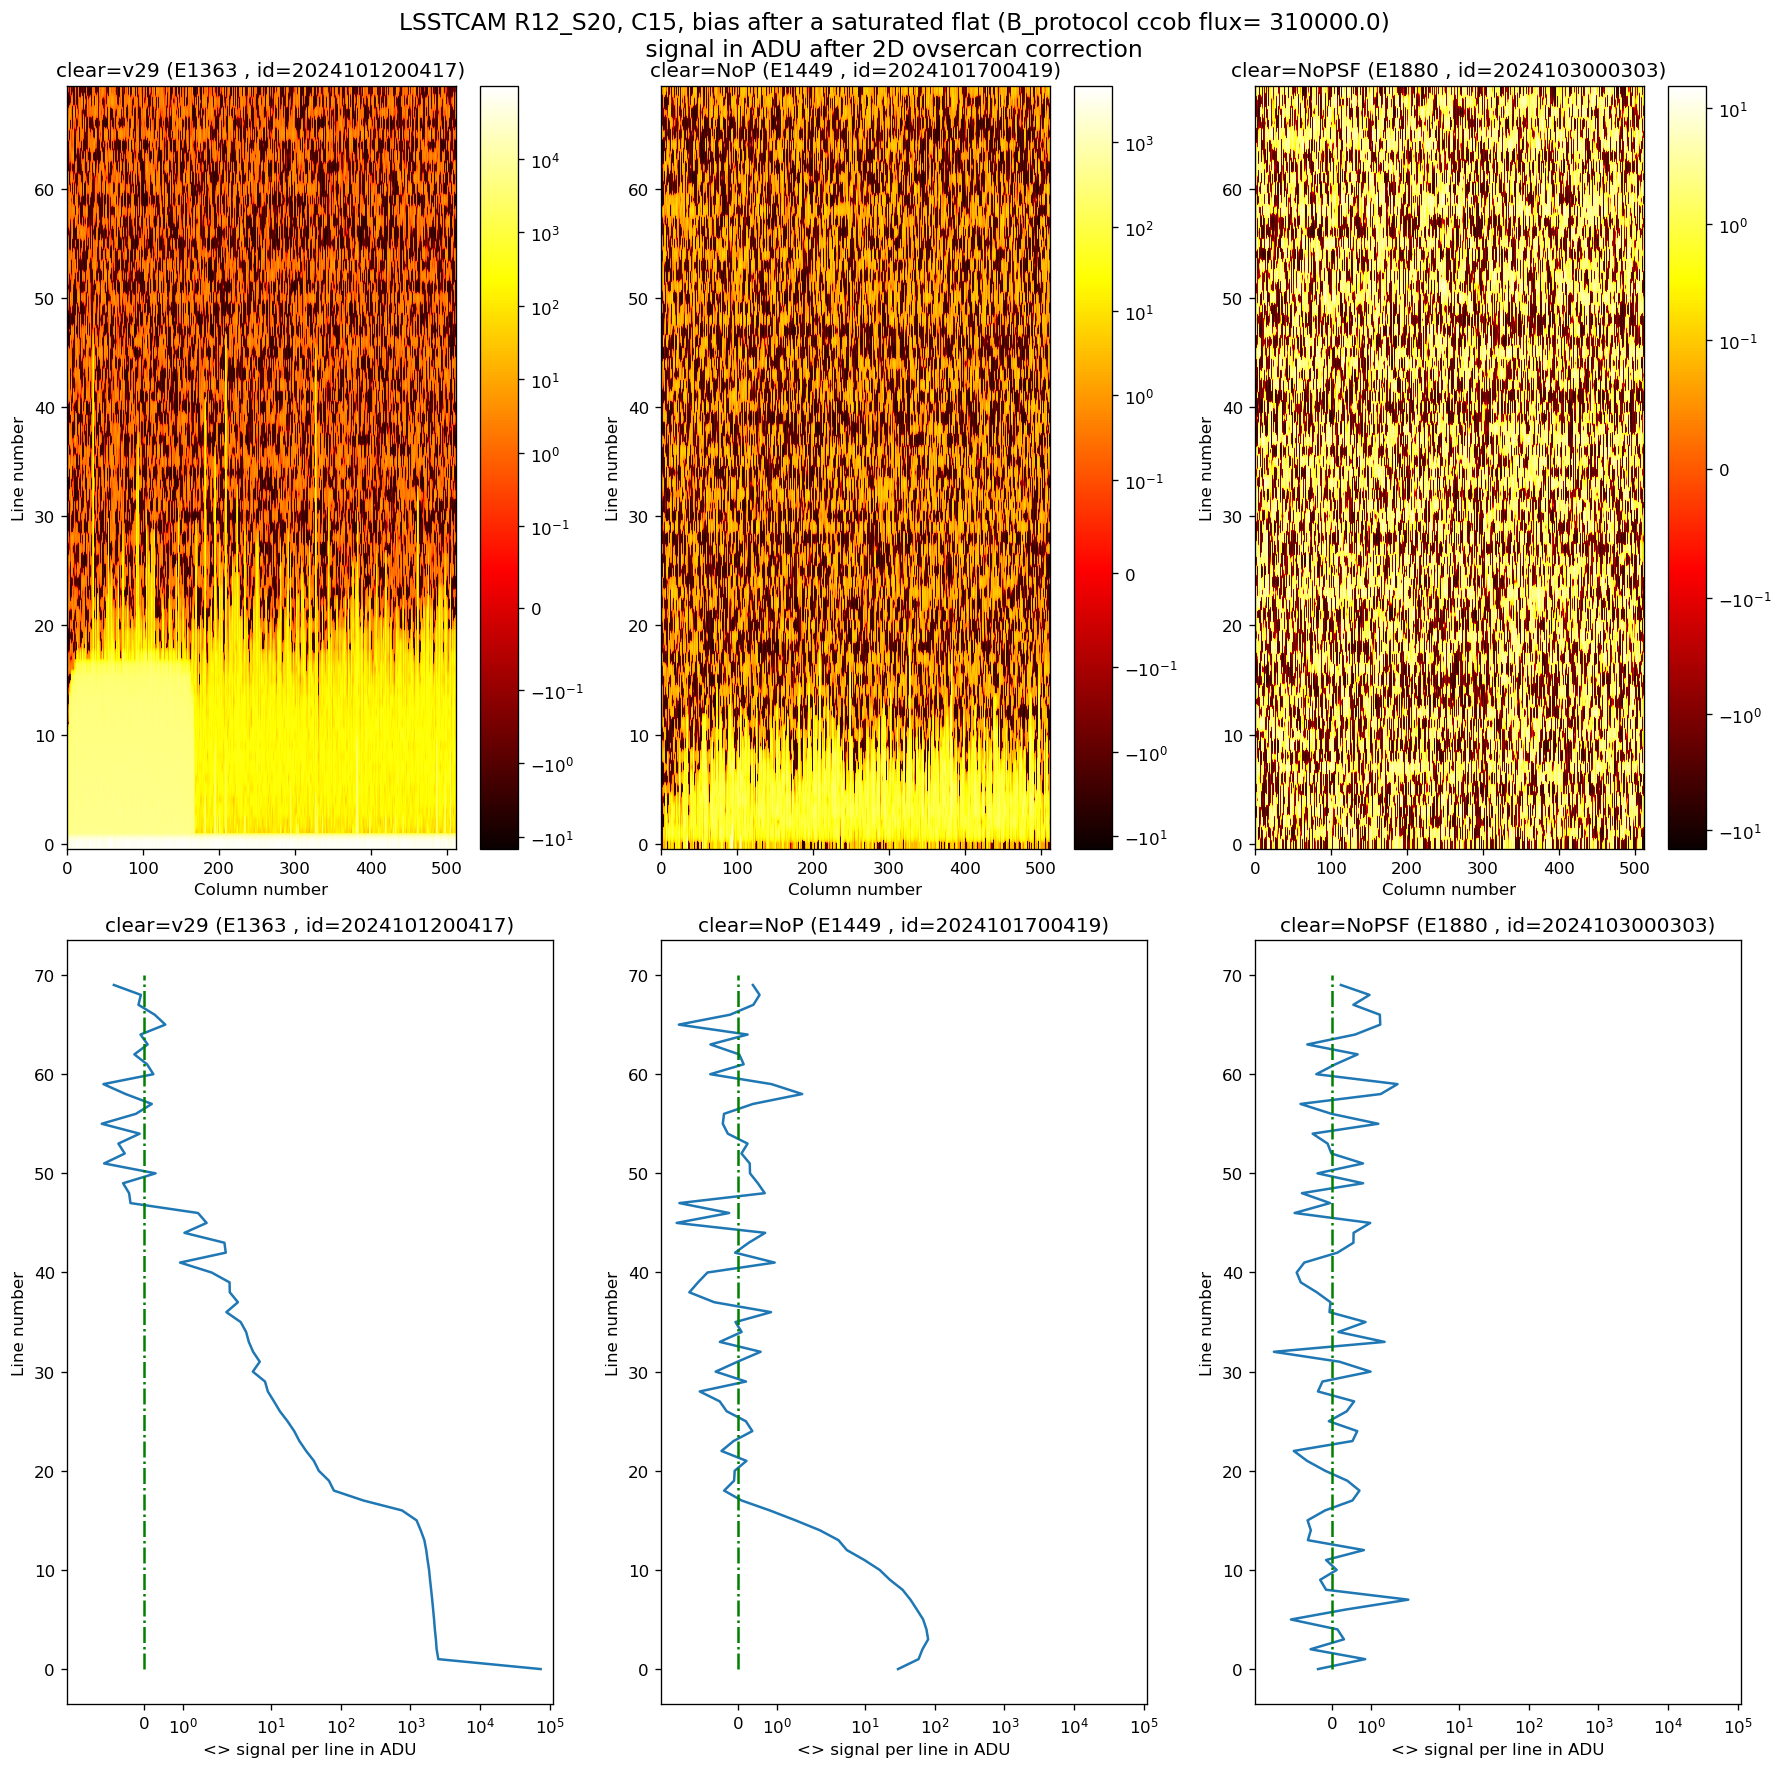
\includegraphics[width=0.9\textwidth]{figures/plots_R12_S20_C15_E1880_bias_2024103000303.png}
\end{centering}
\caption{Impact of the three types of clear on a bias
taken after a saturated flat for an e2v sensor (R12\_S20).
The three panels on top show the interface region between the imaging section and the serial register. The aspect ratio is not 1 for presentation purpose; the bottom three plots are the averaged column profiles.}
\label{fig:clear_e2v}
\end{figure}

%\emph{Figure showing the impact of the various types of clear on a bias
%taken after a saturated flat for an e2v sensor.}



%\emph{Figure showing the impact of the various types of clear on a bias
%taken after a saturated flat for an ITL sensor.}

In Figures~\ref{fig:clear_ITL} and \ref{fig:clear_e2v}, we present for three types of sequencer (from left to
right: V29, Nop, and NopSf), a zoom on the first rows of an ITL or e2v
amplifier (for ITL R03\_S11\_C14 and for e2v
R12\_S20\_C10 shown as a 2D row-columns
image (top plots) or as the mean signal per rows for the first row
read of an amplifier (bottom plots).

As seen in the left-hand panel of Figure~\ref{fig:clear_e2v}
for an e2v CCD, a bias taken just after a saturated flat will show a
residual signal in the first lines read when using the default clear
(left images, clear= V29): the first row has an almost saturated signal
($\sim$100 kADU here), and a significant signal is seen up
to row \textasciitilde50. In practice, depending on the 
amplifier, signal can be seen up to row 20--50. When using the Nop clear
(central plots), we can already see a strong reduction of the uncleared
charges in the first acquired bias after a saturated flat.  Still a small
residual signal is visible in the first $\sim$ 20 rows. The
NopSf clear (right plots) fully clears the saturated flat, and no
uncleared charges are observed in the following bias.

As seen in the left-hand panel of Figure~\ref{fig:clear_ITL}
for an ITL CCD, a bias taken just after a saturated flat will show a
residual signal in the first rows read when using the default clear
(left images, clear=v29): the first row has an almost saturated signal
($\sim$ 100 kADU here), and a significant signal is seen in
the following row. Both Nop clear (central plots) and NopSf clear
(right plots) fully clear the saturated flat, and no uncleared charges
are observed in the following bias image.

\paragraph{An exceptional case: ITL R01\_S10}\label{results-on-itl-r01s10}

\begin{figure}[ht]
\begin{centering}
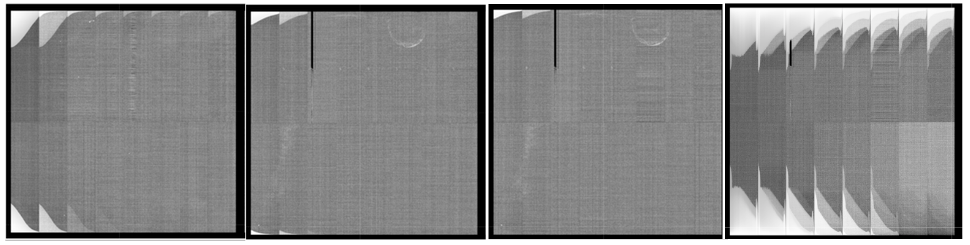
\includegraphics[width=0.95\textwidth]{figures/Clear_R01_S10.png}
\end{centering}
\caption{Impact of the various types of clear on ITL
R01\_S10 after a saturated flat (bias after a saturated flat), from left
to right: 1 standard clear, 3 standard clears, 5 standard clears, 1 Nop
clear, 1 NopSf clear.}
\label{fig:clears_R01_S10}
\end{figure}

%\emph{Figure showing the impact of the various types of clear on ITL
%R01\_S10 after a saturated flat (bias after a saturated flat), from left
%to right: 1 standard clear, 3 standard clears, 5 standard clears, 1 Nop
%clear, 1 NopSf clear}

One ITL sensor, R01\_S10,
presents a specific behavior that is not understood:

\begin{itemize}
\tightlist
\item
  It has a quite low full well (2/3 of nominal).
\item
  The 3 CCDs of this REB (REB1) have a gain 20\% lower than all other ITL CCDs.
\item
  The images taken after a large saturation, as seen in Figure~\ref{fig:clears_R01_S10},
  show a large amount of uncleared charge (with the standard clear: 4
  amplifiers retain \textasciitilde500 rows of saturated signal!).
\end{itemize}

It appears that setting S3 low during the clear as done in Nop and NopSf,
is even worse than a standard clear. This is strange, as a full frame
read, which does this too, manages to clear a saturated image. We notice
that NopSf is \textasciitilde50\% better than Nop, but still worse than
the standard clear, in particular for the 12 amplifiers that are almost correct
with the standard clear.

At this time we do not have a correct way to clear this
sensor once the CCD heavily saturates by uniform illumination, but it is not
clear yet if a saturated star in this sensor, leaving signal in the
parallel overscan, will present the same clear issue.

\paragraph{Conclusion on clears}\label{conclusion}
For e2v sensors, Run 7 finds the NopSf clear fully clears the leftover electrons at the image and the serial register interface.
The NopSf clear grants that the first 50 rows of e2v CCDs that had leftover electrons from the previous exposure are now free of such contamination. NopSf will be the default clear method.

For the ITL sensors, the improvement is still needed even if Nop or NopSf overcome the clear issue because there is the significant exception of R01\_S10 that prevented the usage of those sequencers for ITL devices for Run 7. Note that
aside from R01\_S10 the numbers of lines potentially
``not cleared" in ITL devices after saturated images are small (2 first rows), and they
correspond to a CCD area that is difficult to use anyway (sensor edges with low
efficiency). So at this stage the original clear for ITL remains our default
for ITL, i.e., serial phase 3 always, slightly extended in time to match the NopSf e2v clear execution time, will stay the default method.  Further studies to overcome the problem with
R01\_S10 are foreseen (e.g., investigation of using a continuous
serial flush during exposure at low rate, 10$^6$ pixel flushes in 15\,s).

\subsubsection{Not toggling the RG bit during parallel transfer for e2v sensors}\label{noRGe2v}
During parallel transfer, protecting the CCD amplifier from large signal injection associated with the parallel clock swing is commonly done by activating the Reset Gate (RG) of the CCD amplifier. Although our initial default configuration, following ITL and e2v vendors' practice at the time, this ``RG protection" was not active during the last parallel clock swing.  This was because 
following a dedicated investigation of ITL devices two years ago we found that keeping the RG active during the full parallel transfer provided a clear improvement in the biases \citep{2024SPIE13103E..0WU}. 
By analogy drawn with this ITL study and noticing that today Teledyn e2v, in its current documentation, also recommends to keep the  RG active during the full parallel transfer, such approach  became an area of interest for e2v devices as well. 

At the end of Run 7, two runs ({\it E3578} and {\it E3628}) were collected using, for the e2v devices, the  sequencer {\bf V30\_NoRG}  which activates the Reset Gate during the full parallel transfer. 

Although this was a limited data set a few observations can be made: 
\begin{itemize}
    \item  1D overscan bias corrected image , as they still show 2D structure , are the best place to see first order  2D shape change for various sequencer. For 1D overscan bias correction (serial bias overscan correction only), for detectors with large  bias residuals, a clear improvement (\textasciitilde2 ADU = \textasciitilde 30\% reduction) has been observed with the {\bf V30\_NoRG} sequencer compared to the {\bf V30} one (Figure~\ref{fig:1DNoRGEffect}).
    \item For 2D overscan corrected images, no improvement was found in the stability of the bias shape with exposure time.  
    \item For 2D overscan bias correction, leftover bias structures  are unchanged between  sequencer {\bf V30} and sequencer {\bf V30\_NoRG} (Fig.~\ref{fig:2DNoRGEffect}).

\end{itemize}

So in practice running with {\bf V30\_NoRG} sequencer  reduces the amplitude of the 2D bias shape of the biases: 2D residuals are smaller after 1D overscan bias correction.  This confirms that part of the 2D bias shape in e2v sensors is related to parallel clock usage during readout. 

Nevertheless if the biases' 2D shape is reduced, it is still present when using {\bf V30\_NoRG} sequencer, and the corresponding issues in the removal of this 2D shape are unchanged : 
\begin{itemize}
\item The 2D overscan bias correction  presents  up to \textasciitilde1 ADU bias residual in some amplifiers (Figure~\ref{fig:2DNoRGEffect}): unfortunately there is no improvement when using  {\bf V30\_NoRG} sequencer in those 2D bias residuals. 
\item Also the {\bf V30\_NoRG} sequencer will not be the solution to remove the dependency of the 2D bias shape with the exposure time (Figure~\ref{fig:BiasVSDark}).
\end{itemize}

\begin{figure}[ht]
\begin{centering}
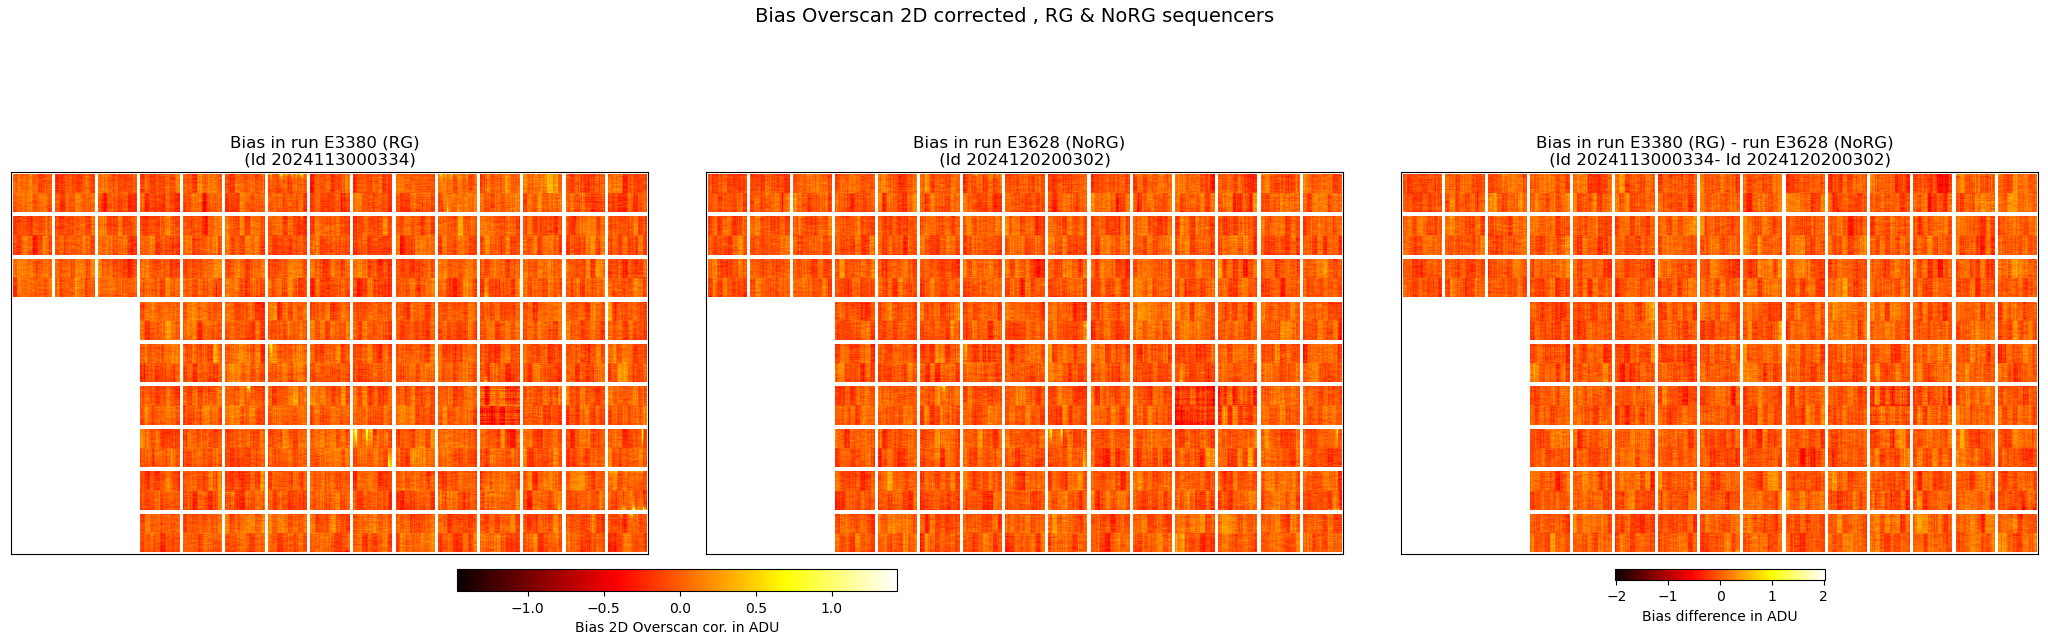
\includegraphics[width=0.9\textwidth]{figures/Bias_PA_2D_raw_RG_NoRG_2024113000334_2024120200302.png}
\end{centering}
\caption{For e2v sensors , biases residuals after a 2D overscan correction : left plot, bias in run {\it E3380} collected  with sequencer {\bf V30}), central plot, bias in run {\it E3628} collected with sequencer {\bf V30\_NoRG}, right plot the difference of the two biases :  No obvious difference is observed.}\label{fig:2DNoRGEffect}
\end{figure}

\begin{figure}[ht]
\begin{centering}
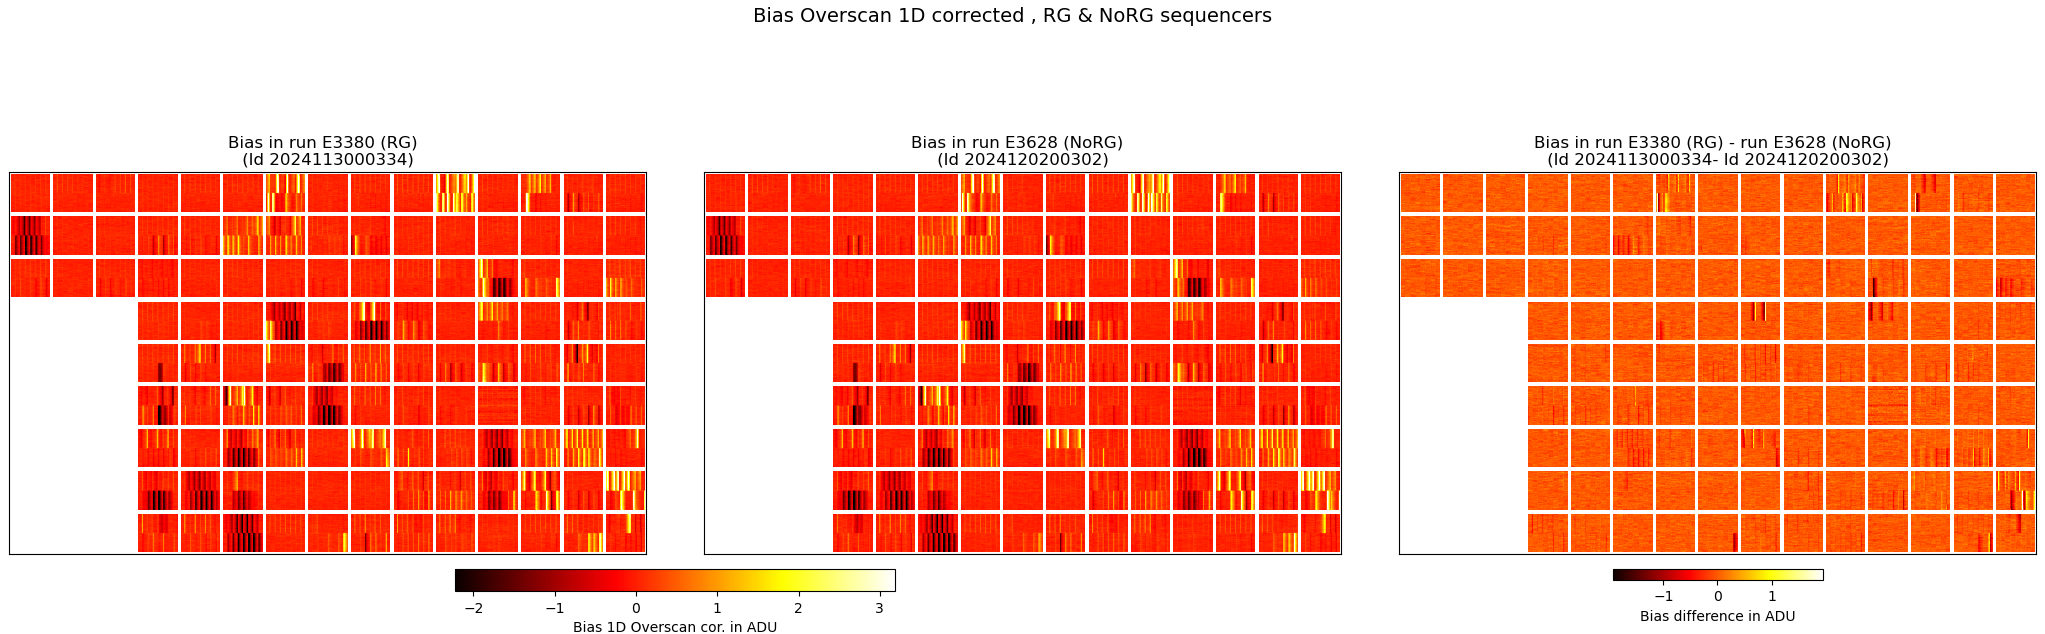
\includegraphics[width=0.9\textwidth]{figures/Bias_PA_1D_raw_RG_NoRG_2024113000334_2024120200302.png}
\end{centering}
\caption{For e2v sensors , biases residuals after 1D overscan correction : left plot, bias in run {\it E3380} collected  with sequencer {\bf V30}), central plot, bias in run {\it E3628} collected with sequencer {\bf V30\_NoRG}, right plot the difference of the two biases : \textasciitilde40 amplifiers show a smaller (1--2 ADU)  bias residual level in  the case of the {\it NoRG} sequencer run. }\label{fig:1DNoRGEffect}
\end{figure}

\begin{figure}[ht]
\begin{centering}
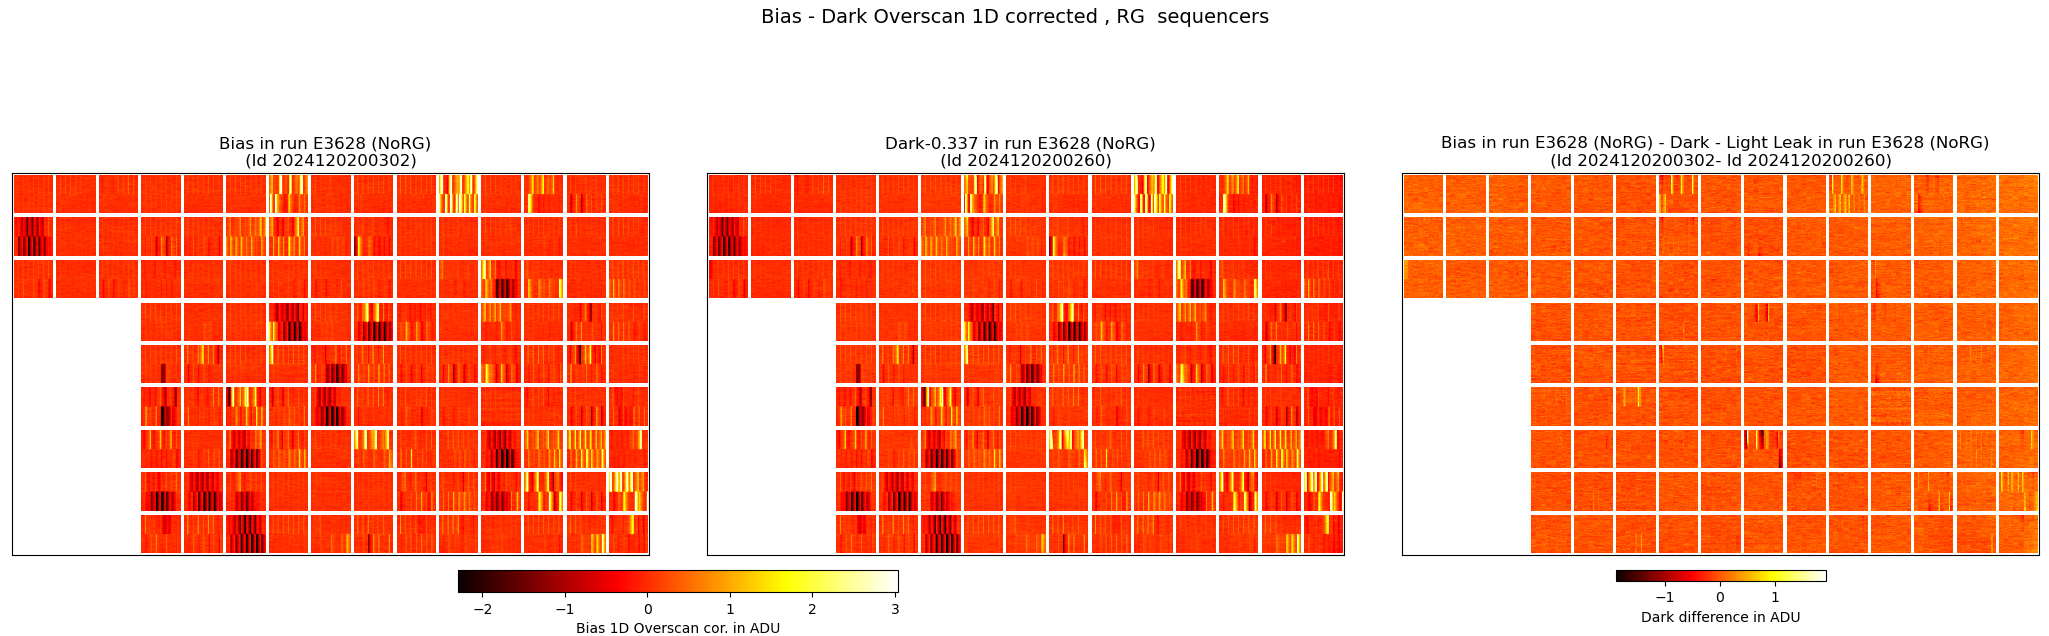
\includegraphics[width=0.9\textwidth]{figures/1D_raw_NoRG_E3628_Bias-Dark_2024120200302_2024120200260.png}
\end{centering}
\caption{For 1D overscan corrected biases, here from {\it E3628} collected with sequencer {\bf V30\_NoRG}, we observe that the 2D shape is still function of the exposure length : on the left we have a Bias , in the center a 15s Dark (corrected for light leak) and on the right the difference : up to \textasciitilde+/-1 ADU residuals difference are observed for a few amplifiers. Notice that this has been identified as a change in bias structure in function of the exposure time and is unrelated to dark current that are negligible for those exposure times. This is similar to what we observed in run {\it E3380} collected  with sequencer {\bf V30}) }\label{fig:BiasVSDark}
\end{figure}

\clearpage

\subsubsection{Disabling IDLE FLUSH}\label{section:disablingIDLEFLUSH}

IDLE\_FLUSH is one of the ``mains" settings in the sequencer file that enables the sequencer output to run while in the IDLE state (the period between one exposure and the next). The specific implementation of IDLE\_FLUSH can be selected from various functions in the sequencer file. In Run 5, we chose the \texttt{ReadPixel} function, which reads out a pixel. This choice was initially made to mitigate the so-called yellow corner issue, a 2D structure of elevated signal near an amplifier corner observed in bias and dark exposures for certain amplifiers on e2v CCDs (see details in \citet{2024SPIE13103E..0WU}).

However, it was reported that running IDLE\_FLUSH exacerbates the divisadero tearing issue. Divisadero tearing appears as a signal deficiency at amplifier boundaries in e2v sensors, accompanied by increased signal in adjacent columns. Additionally, using \texttt{ReadPixel} as the IDLE\_FLUSH function has the greatest thermal impact because it continuously operates the Analog-to-Digital Converter at its maximum rate. This results in a significant difference in power consumption, more than 50\,W over all rafts, between the exposure state and the IDLE state. Consequently, the focal plane experiences a temperature variation of approximately 2~deg C between periods of image acquisition and idle periods (Figure~\ref{fig:IdleFlushEffect}).

\begin{figure}[ht]
\begin{centering}
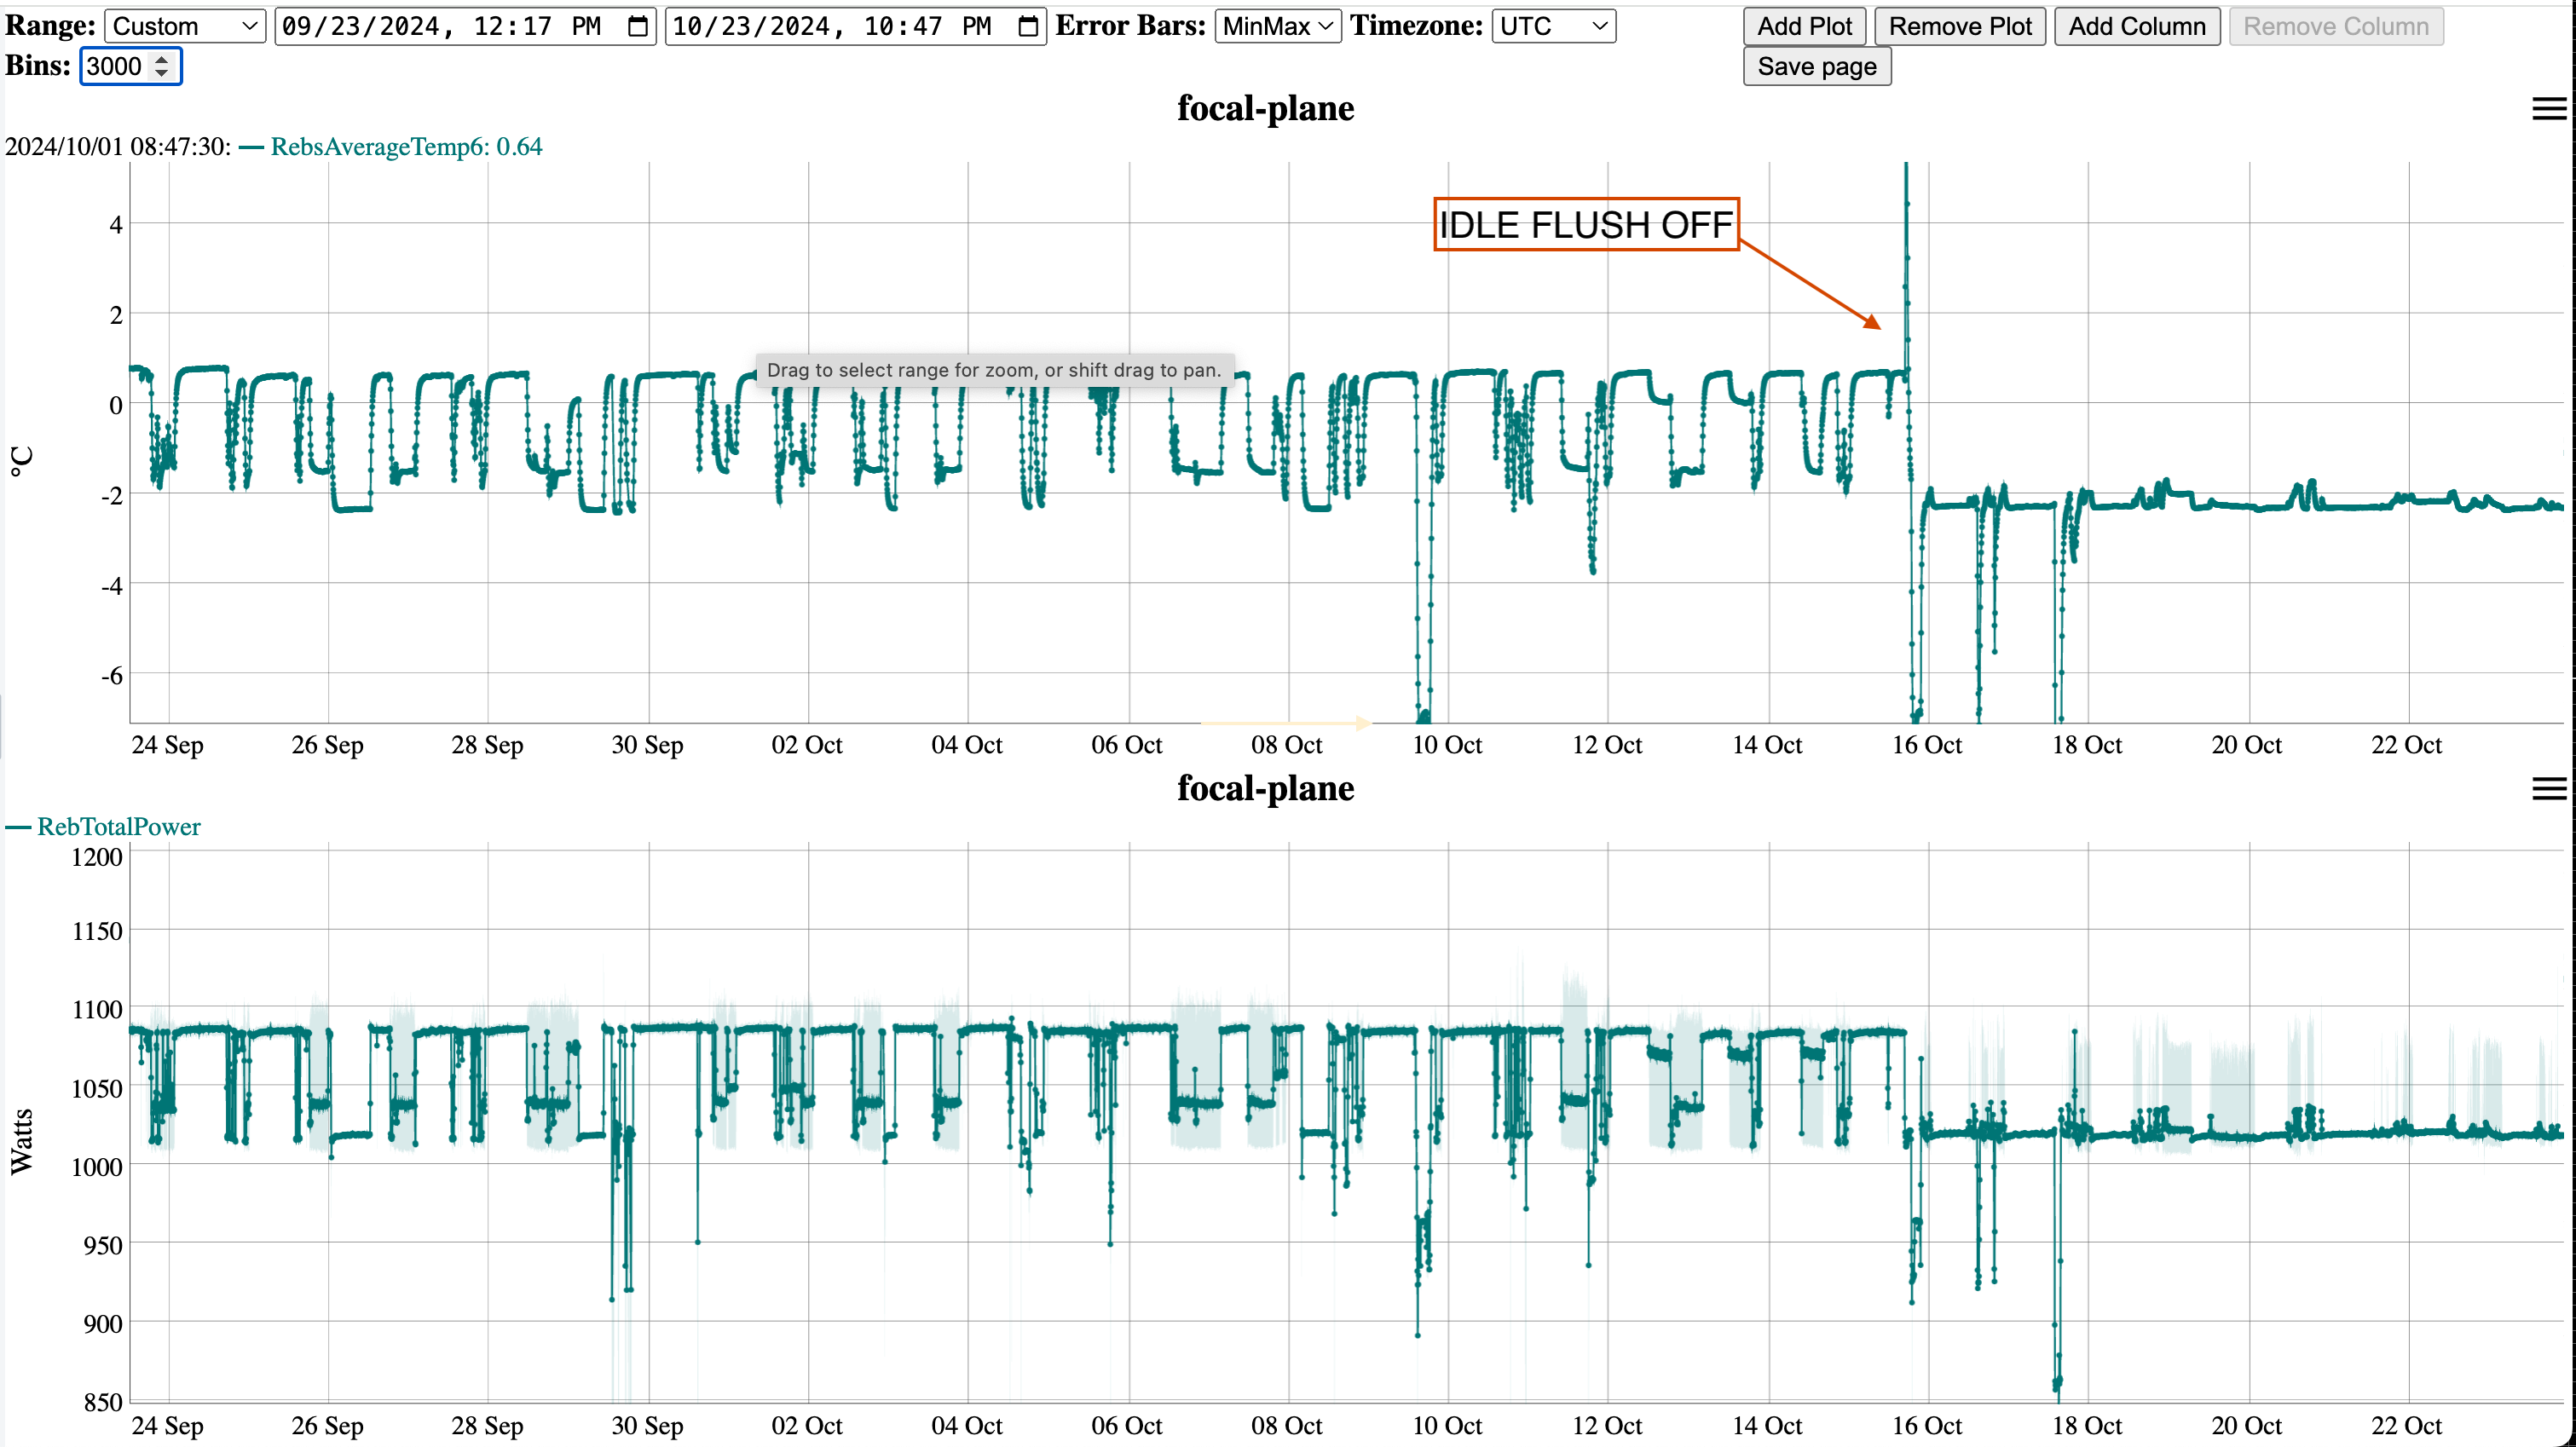
\includegraphics[width=0.9\textwidth]{figures/REB_power_temp6_sept24_to_Oct23.png}
\end{centering}
\caption{Impact of enabling and disabling IDLE\_FLUSH on focal-plane temperature and power consumption.}\label{fig:IdleFlushEffect}
\end{figure}

This temperature variation in the focal plane can lead to changes in the REB temperature, potentially causing gain variations or instability in the bias. Based on these considerations, we decided to disable IDLE\_FLUSH. The impact of this change on bias stability is discussed in Sections~\ref{sec:bias-stability-2} and~\ref{sec:gain-stability-2}.

\begin{figure}[ht]
\begin{centering}
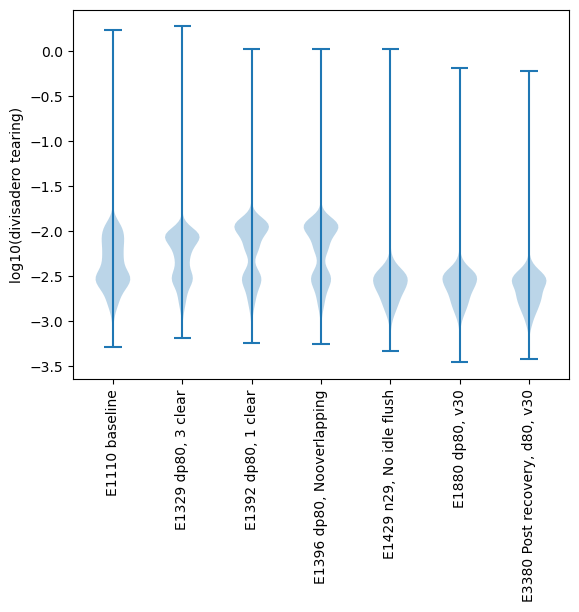
\includegraphics[width=0.5\textwidth]{figures/divisadero.png}
\end{centering}
\caption{Impact of disabling IDLE\_FLUSH on divisadero tearing metric.}\label{IdleFlushEffect:divisadero}
\end{figure}

Figure \ref{IdleFlushEffect:divisadero} shows the impact on the divisadero tearing. Shown there are selected B protocol runs with different settings in chronological order. A few changes of settings were tested: (1) switching to narrower parallel swing voltage, (2) changing the number of clears before the exposure, (3) disabling IDLE\_FLUSH.  Some runs with these different settings also included some minor additional changes in settings, or a change of the sequencer file (the change from v29 to v30  is primarily incorporation of the change in the number of clears). The figure includes both ITL and e2v results. The two distinct distributions in earlier runs correspond to the differences between the two types of CCD (the upper one is e2v and the lower one is ITL). The greatest change can be seen when we switched to not running IDLE\_FLUSH at E1429, which brought down the overall distribution. The two distributions became indistinguishable, which indicates that the majority of the divisadero tearing for e2v is mitigated.

E3380 was the run taken after the recovery from the shutdown due to poor performance of the Pumped Coolant System (see Sec. \ref{ganttchart}). The stability of the results confirms that the metric is consistent across power cycling of LSSTCam.

\subsection{Summary}\label{summary:optimization}

All e2v sensors exhibited persistence in dark images acquired after images with bright illumination. We confirmed that reducing the parallel swing voltage of the e2v CCD operation greatly reduced persistence. As penalties, we observed a full well reduction of 23\% and a \textasciitilde10\% increase of the
brighter-fatter effect in the area coefficient, essentially in an isotropic way.

Sequencer files have undergone evolution for both ITL and e2v versions.
The final sequencer file from Run 6 was the
v26noRG version for ITL and the regular v26
for e2v. The suffix noRG indicates that the
RG bit is not toggled during parallel transfer. This modification
enhances the stability of the bias structure for most ITL
amplifiers.

During Run 7, several changes were implemented, as described below:

\begin{itemize}
\tightlist
\item
  v27 incorporated guider functionalities, including ParallelFlushG and
  ReadGFrame. However, the noRG change was inadvertently included.
  Consequently, we abandoned this version and switched to v28.
\item  \href{https://rubinobs.atlassian.net/browse/LSSTCAM-5}{v28 sequencer files merged v26noRG and
  v27.}
\item\href{https://rubinobs.atlassian.net/browse/LSSTCAM-34}{v29 introduced changes to speed up the guider readout.}
\item
  \href{https://github.com/lsst-camera-dh/sequencer-files/pull/17}{v30 primarily focused on e2v}. We introduced NopSf
  for e2v CCDs. \href{https://github.com/lsst-camera-dh/sequencer-files/pull/18}{Timing of the e2v version is modified to align with the ITL version.}
\end{itemize}

We also disabled IDLE\_FLUSH to improve the thermal situation and the divisadero tearing.

\clearpage